\documentclass[11pt,a4paper]{article}

\usepackage[T1]{fontenc}
\usepackage[utf8]{inputenc}
\usepackage{amsmath,amssymb,booktabs,geometry,graphicx,hyperref,microtype}
\usepackage[british]{babel}
\geometry{margin=2.5cm}
\hypersetup{colorlinks=true,linkcolor=black,urlcolor=blue}

\title{Demand, Regionality, Entry Selectivity, and the Research Talent Pipeline in Portuguese Higher Education}
\author{Diogo}
\date{26 August 2026}

\begin{document}
\maketitle

\begin{abstract}
This study evaluates three empirical propositions about Portuguese higher education:
whether placements in science and engineering are declining; whether student choice
is predominantly regional and demand pressure accounts for cross-institution
differences in entry grades; and whether high-performing research units are exposed
to a weakening educational pipeline. The empirical analysis addresses the first
proposition and begins the demand/selectivity component of the second. Comparable
broad-area first-phase tables are observed for 2017, 2018 and 2020--2026; no 2019
field value is reconstructed. Registered STEM placements rise from 13,926 in 2017 to
15,181 in 2026 (+9.0\%), while their share of all first-phase placements falls by 0.64
percentage points. A demographic sensitivity using an average single-year cohort proxy
reduces the all-STEM endpoint change to +1.3\%, with strong component heterogeneity.
Separately, a matched panel fixes DGES course 9119 (Engenharia Informática) across 23
institutions in 2018--2020. Within year, log applicants per vacancy accounts for
55.9--74.3\% of cross-institution variation in the general-contingent cut-off and
49.8--76.6\% of variation in the mean application grade of placed candidates.
Institution effects absorb much persistent structure, but demand still improves
leave-one-year-out prediction. Neither analysis is generalised beyond its measured
scope: the historical programme-level STEM test, regionality, rankings and the R\&D
pipeline remain separate evidence tasks.
\end{abstract}

\section{Introduction}
Portuguese public discussion about higher education often combines three levels of
analysis: immediate admission outcomes, the geography and selectivity of student
choice, and the long-run supply of researchers. These levels are related, but they
are not interchangeable. This paper constructs a unified empirical framework in
which each can be measured separately before their connections are examined.

The analysis is proposition-neutral. A public claim is translated into observable
estimands and can receive supportive, contradictory, mixed, or insufficient evidence.
Descriptive, predictive, associational, and causal language are kept separate. The current evidence concerns science and engineering placements and a matched-course
demand/selectivity pilot; regionality, rankings and the research-pipeline question
remain independently specified.

\section{Empirical propositions}
\subsection{Science and engineering placements}
The first proposition is that placements in science and engineering have entered a
sustained decline. A meaningful evaluation must separate realised placements from
applicant demand, first preferences, places offered, occupancy, field share and
population scale. A decline on one margin need not imply decline on the others.

\subsection{Regionality, demand pressure, and entry grades}
The second proposition has three components: that higher-education choice is strongly
regional; that applicants per place account for most differences in entry grades; and
that ranking information has little incremental explanatory value. These questions
are analysed separately to avoid conflating geography, demand, selectivity and
reputation.

\subsection{The R\&D talent pipeline}
The third proposition is that high-performing research units may face future
constraints when the educational pipeline feeding their fields and host institutions
weakens. Because future capacity constraints are not always directly observable, the
design distinguishes current pipeline exposure from realised downstream research
outcomes.

\section{Data}
The full study uses official Concurso Nacional de Acesso (CNA) statistics, DGEEC
RAIDES and science-and-technology statistics, FCT R\&D-unit evaluations, and official
demographic data. Historical ranking information is an optional secondary layer.

The CNA archive is treated as a sequence of historical source formats rather than as
one immutable schema. The long-run target is 1997--2026. For a future
institution--programme panel, applicant and grade statistics are kept distinct from
capacity and cut-off tables, and duplicated placement counts can be used as
cross-source consistency checks. Historical mobility geography is preserved rather
than silently coerced into modern district labels.

\subsection{Broad-area first-phase tables}
The present medium-run analysis uses complete official broad-area first-phase tables
for 2017, 2018 and 2020--2026. The 2017 official document labels the relevant table
\emph{Quadro XII}; later observed vintages use \emph{Quadro V}. Each observed year
contains 23 broad study areas with vacancies, first-choice candidates, placements and
remaining vacancies.

The official 2019 first-phase statistical index lists a placement summary,
establishment and course comparisons, mobility, cut-offs and programme-pair
statistics, but it does not list a comparable complete broad-area placement table.\footnote{Direcao-Geral do Ensino Superior, \href{https://www.dges.gov.pt/guias/pdfs/statcol/2019/}{2019 CNA statistical archive}.}
National 2019 totals therefore cannot identify field composition, and no broad-area
observation is interpolated or inferred from neighbouring years.

For every observed year, the broad-area data satisfy
\[
\sum_g V_{gt}=V_t,\qquad
\sum_g A^{(1)}_{gt}=A_t,\qquad
\sum_g P_{gt}=P_t,
\]
before STEM aggregation. The nine observed years therefore contribute
$9\times23=207$ area-year observations.

\subsection{Demographic series}
The preferred denominator for the final access-rate analysis is population aged
exactly 18. A source-locked single-age series is not yet available in the present
dataset. The demographic sensitivity therefore uses the INE resident population aged
15--24 disseminated by PORDATA.\footnote{PORDATA, \href{https://www.pordata.pt/en/portugal/resident+population+of+working+age+total+and+by+age+group-3245}{resident population by age group}; source entity INE, last updated 22 June 2026.}
The observed 15--24 population rises from 1,101,839 in 2016 to 1,185,234 in 2025,
which is a 7.6\% increase between the population references used for the 2017 and
2026 admission endpoints.


\subsection{Matched-course comparative statistics}
For the first demand/selectivity analysis, two official DGES comparative course
publications are used: the 2018--2019 and 2019--2020 first-phase tables.\footnote{Direcao-Geral do Ensino Superior,
\href{https://www.dges.gov.pt/guias/pdfs/statcol/2019/StatsCurso19.pdf}{course statistics 2018--2019} and
\href{https://www.dges.gov.pt/guias/pdfs/statcol/2020/StatsCurso20.pdf}{course statistics 2019--2020}.}
The design fixes course code 9119, \emph{Engenharia Informatica} [Licenciatura], and
retains the same 23 institutions in 2018, 2019 and 2020. The tables report vacancies,
total and first-choice applicants, total and first-choice placements, the
general-contingent cut-off and mean grade components.

The two publications both report 2019. The 23 repeated institution-course records are
therefore compared measure by measure before deduplication. Every duplicated count and
grade agrees exactly, yielding a balanced analytical panel of 69 institution-year
observations.

\section{Methods}
\subsection{Access and placement}
For field group $g$ and competition year $t$, define placement share
\[
S_{gt}=\frac{P_{gt}}{P_{\cdot t}},
\]
occupancy
\[
O_{gt}=\frac{P_{gt}}{V_{gt}},
\]
and first-choice pressure
\[
F_{gt}=\frac{A^{(1)}_{gt}}{V_{gt}}.
\]
The broad-area table reports first-choice candidates, not total applications, so
$F_{gt}$ is not relabelled as applicants per vacancy. The programme-level analysis
will separately use total applicants per vacancy.

The STEM grouping contains three broad ISCED-F-compatible components: 05, natural
sciences, mathematics and statistics; 06, information and communication technologies;
and 07, engineering, manufacturing and construction. The seven published source
areas beneath those components are retained before aggregation.

\subsection{Medium-run descriptive paths}
For each component and the all-STEM aggregate, the fitted count description is
\[
\log P_{gt}=\alpha_g+\beta_g t+e_{gt}.
\]
The annual percentage path is reported as $100[\exp(\widehat\beta_g)-1]$.
Placement share, occupancy and first-choice pressure are summarised by linear
percentage-point gradients in calendar year. Calendar year itself is the regressor,
so the missing 2019 observation remains a two-year interval between 2018 and 2020.
For the same reason, the movement from 2018 to 2020 is not labelled a year-on-year
change.

A pre-specified sensitivity excludes 2020 and 2021. These observations are
administrative population counts rather than a probability sample, and nine observed
years are too few for credible data-driven break selection. The fitted slopes and
$R^2$ values are therefore descriptive summaries; no sampling p-values or causal
interpretation are attached to them.

\subsection{Broad-cohort demographic sensitivity}
Let $N_{15:24,t-1}$ denote the resident population aged 15--24 in the calendar year
preceding competition year $t$. The sensitivity defines an average single-year cohort
proxy
\[
C^{\mathrm{proxy}}_t=\frac{N_{15:24,t-1}}{10},
\]
and the normalised placement rate
\[
H_{gt}=1000\frac{P_{gt}}{C^{\mathrm{proxy}}_t}.
\]
This denominator is deliberately weaker than an exact age-18 count. It is used only
to test whether endpoint changes in placements are commensurate with the scale of the
relevant young-adult population. Raw counts and national placement shares remain
separate outcomes.

\subsection{Regionality and entry grades}
Let $F_{odt}$ denote first-choice flow from access-origin area $o$ to destination
district $d$. Historical source geography is not assumed homogeneous: older CAE/GAES
origins can be access areas rather than districts. For origins genuinely comparable
to destination districts or autonomous regions, the same-area share is
\[
R_t=
\frac{\sum_{d\in\mathcal{C}_t}F_{ddt}}
{\sum_{o\in\mathcal{C}_t}\sum_d F_{odt}}.
\]
Entropy, mutual information and, where appropriate, a gravity-style model supplement
the diagonal share.

The matched-course demand pilot defines
\[
D_{jt}=\frac{A_{jt}}{V_{jt}},
\]
where $A_{jt}$ is total applicants and $V_{jt}$ initial vacancies for institution $j$.
Within each year, the descriptive association is
\[
y_{jt}=\alpha_t+\beta_t\log D_{jt}+e_{jt}.
\]
Nested pooled descriptions add a linear year term, demand and institution fixed
effects in sequence. The same specifications are assessed by holding out each complete
year. Reported quantities are coefficients, $R^2$, incremental $R^2$, RMSE and MAE;
they are not treated as causal or sampling-inference statistics. Rankings enter only
after the broader geography/demand panel exists.

\subsection{R\&D pipeline exposure}
R\&D units are linked to host institutions and feeder fields through explicit weights.
Pipeline stages are measured separately from first-time entry through doctoral output
and research personnel. Composite risk indices, if used, are exploratory and
accompanied by component-level results.

\section{Study A results}
\subsection{All-STEM path}
Table~\ref{tab:annual} reports the observed all-STEM series. The missing 2019 row
represents an unobserved field composition, not a zero.

\begin{table}[htbp]
\centering
\caption{Registered STEM first-phase broad-area series}\label{tab:annual}
\begin{tabular}{rrrrrr}
\toprule
Year & Vacancies & First choice & Placements & Occupancy & Placement share \\
\midrule
2017 & 16,655 & 14,700 & 13,926 & 83.61\% & 31.01\% \\
2018 & 16,809 & 13,666 & 13,539 & 80.55\% & 30.78\% \\
2020 & 18,971 & 16,225 & 15,886 & 83.74\% & 31.17\% \\
2021 & 18,592 & 15,253 & 14,692 & 79.02\% & 29.71\% \\
2022 & 18,299 & 15,955 & 15,109 & 82.57\% & 30.34\% \\
2023 & 18,355 & 15,082 & 14,984 & 81.63\% & 30.31\% \\
2024 & 18,396 & 15,716 & 15,365 & 83.52\% & 30.75\% \\
2025 & 18,471 & 12,967 & 13,183 & 71.37\% & 30.03\% \\
2026 & 18,730 & 15,103 & 15,181 & 81.05\% & 30.37\% \\
\bottomrule
\end{tabular}
\end{table}

The endpoint count rises by 9.0\%, from 13,926 in 2017 to 15,181 in 2026. The share
of all first-phase placements moves in the opposite direction, from 31.01\% to
30.37\%, a decline of 0.64 percentage points. Raw count and relative field share are
therefore not interchangeable measures of decline.

The all-STEM log-linear fit is weak: the slope corresponds to +0.46\% placements per
calendar year with $R^2=0.050$. The placement-share gradient is -0.077 percentage
points per year. Excluding 2020 and 2021 changes the count slope to +0.75\% per year
and the share gradient to -0.074 percentage points per year. Neither fitted line
explains much of the annual variation.

\begin{figure}[htbp]
\centering
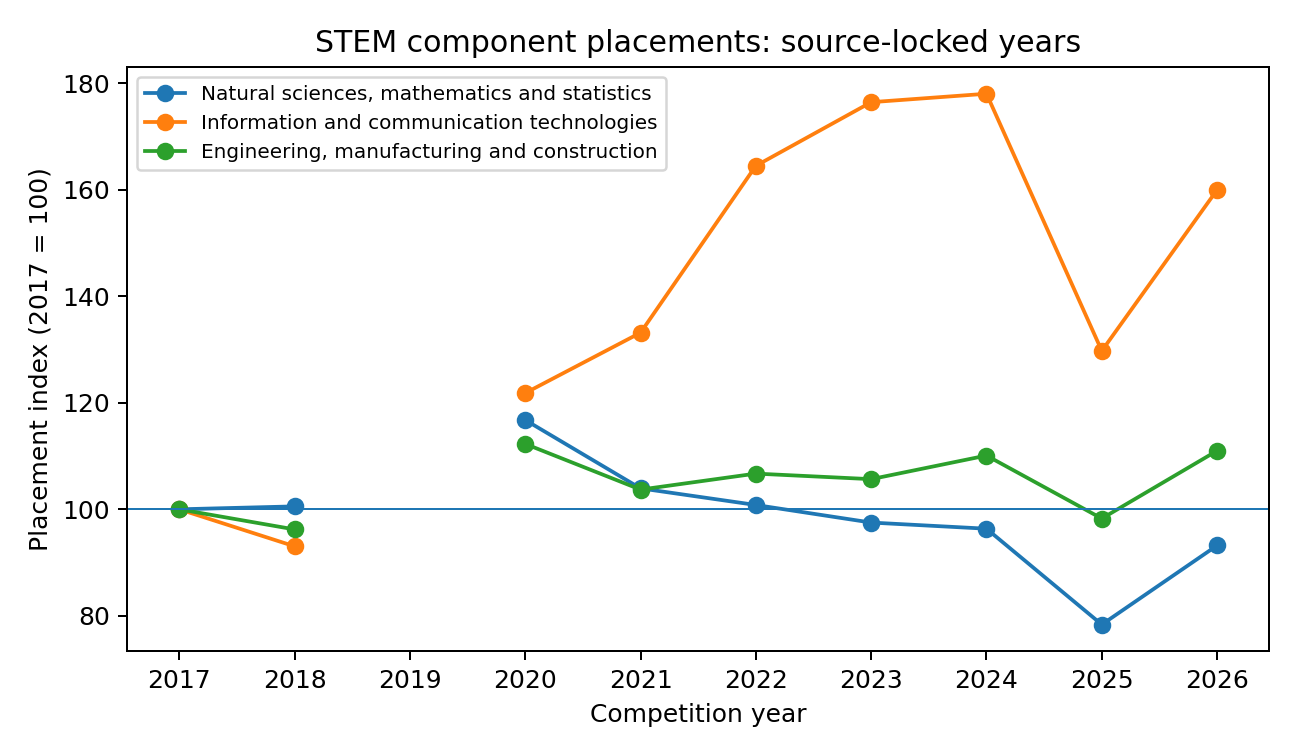
\includegraphics[width=0.86\textwidth]{../figures/study_a/medium_run_component_index.png}
\caption{Placement trajectories by registered STEM component, normalised to 2017 = 100. The 2019 gap denotes an unobserved field-composition year.}
\end{figure}

\subsection{Component heterogeneity}
The all-STEM aggregate masks materially different paths.

\begin{table}[htbp]
\centering
\caption{STEM component endpoint and fitted-path comparison}\label{tab:components}
\begin{tabular}{lrrrr}
\toprule
Component & 2017 & 2026 & Endpoint & Annual path \\
\midrule
Natural sciences, mathematics and statistics & 3,816 & 3,557 & $-6.8\%$ & $-2.0\%$ \\
Information and communication technologies & 820 & 1,312 & $+60.0\%$ & $+6.3\%$ \\
Engineering, manufacturing and construction & 9,290 & 10,312 & $+11.0\%$ & $+0.8\%$ \\
\textbf{All registered STEM} & \textbf{13,926} & \textbf{15,181} & \textbf{$+9.0\%$} & \textbf{$+0.5\%$} \\
\bottomrule
\end{tabular}
\end{table}

Group 05 is the only registered component lower at the 2026 endpoint. ICT is 60.0\%
above its 2017 placement count, while group 07 is 11.0\% above 2017. Within group 07,
the published source category \emph{Engenharia e Tecnicas Afins} rises by 11.7\%
between the same endpoints. The fitted paths reinforce the heterogeneity: group 05
has a -1.99\% annual log-linear count description, ICT +6.29\%, and group 07 +0.79\%.
These are descriptive path summaries, not trend-significance tests.

\subsection{Demographic scale}
The raw endpoint changes and broad-cohort-normalised changes are compared in
Table~\ref{tab:demography}.

\begin{table}[htbp]
\centering
\caption{Raw and broad-cohort-normalised endpoint changes, 2017--2026}\label{tab:demography}
\begin{tabular}{lrr}
\toprule
Component & Raw placements & Cohort-proxy rate \\
\midrule
Natural sciences, mathematics and statistics & $-6.8\%$ & $-13.3\%$ \\
Information and communication technologies & $+60.0\%$ & $+48.7\%$ \\
Engineering, manufacturing and construction & $+11.0\%$ & $+3.2\%$ \\
\textbf{All registered STEM} & \textbf{$+9.0\%$} & \textbf{$+1.3\%$} \\
\bottomrule
\end{tabular}
\end{table}

The all-STEM rate changes from 126.4 to 128.1 placements per 1,000 average single-year
cohort equivalents. Thus most of the +9.0\% raw endpoint increase is commensurate with
the 7.6\% growth of the broad young-adult population reference. The demographic
sensitivity does not reverse the raw-count result, but it changes its magnitude
substantially. It also sharpens the component decomposition: group 05 weakens further
after normalisation, ICT still expands strongly, and group 07 is only modestly above
its 2017 rate.

\begin{figure}[htbp]
\centering
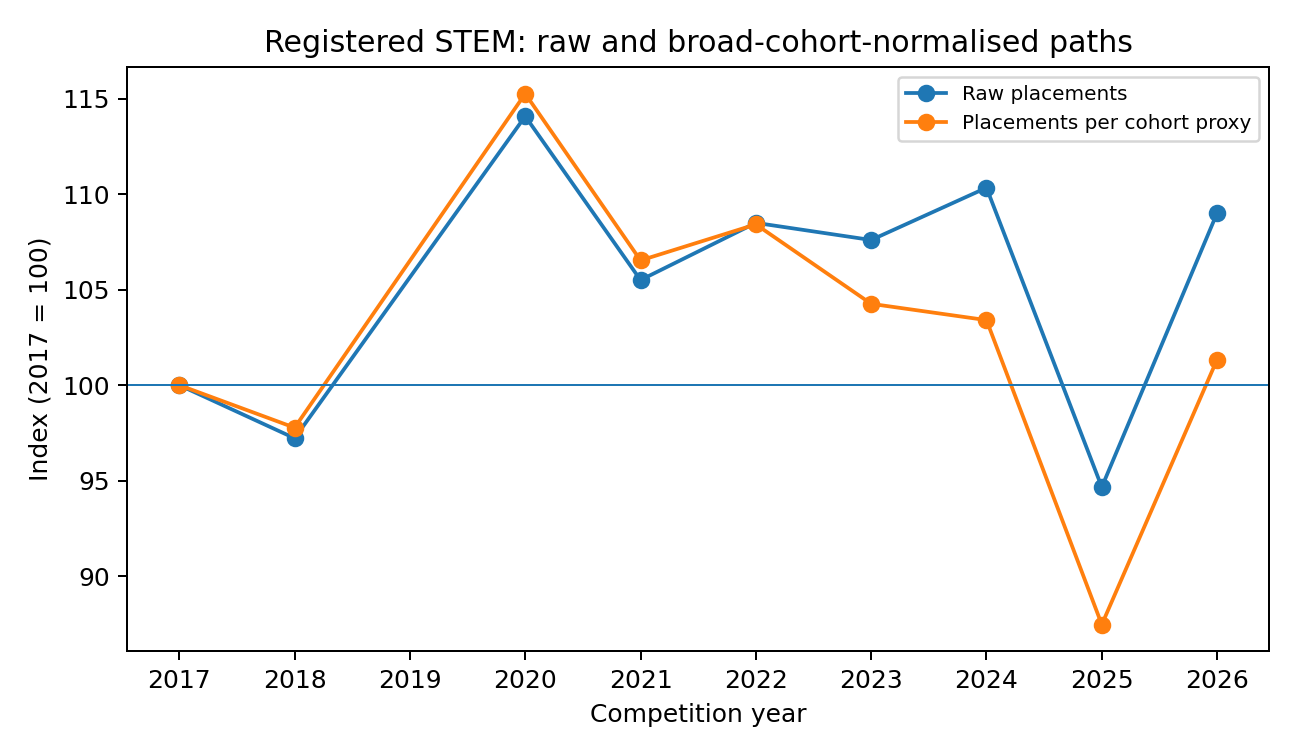
\includegraphics[width=0.82\textwidth]{../figures/study_a/medium_run_demographic_index.png}
\caption{All-STEM raw placements and broad-cohort-normalised placement rates, indexed to 2017 = 100. The demographic denominator is the preceding-year population aged 15--24 divided by ten, not population aged exactly 18.}
\end{figure}

\subsection{The 2025 trough}
The recent window identifies a sharp short-run event. Registered STEM placements fall
from 15,365 in 2024 to 13,183 in 2025 (-14.2\%) and then recover to 15,181 in 2026
(+15.2\%). National first-phase placements show the same broad discontinuity, falling
from 49,963 to 43,899 before recovering to 49,991. The medium-run evidence therefore
treats 2025 as a pronounced trough rather than extrapolating it into a monotonic
historical path.

\section{Study B matched-course pilot}
\subsection{Cross-institution demand association}
For course 9119, applicants per vacancy vary substantially across the 23 institutions.
A single log-demand predictor accounts for a material share of cross-institution grade
variation in each year (Table~\ref{tab:coursepilot}).

\begin{table}[htbp]
\centering
\caption{Year-specific $R^2$ from log applicants per vacancy, course 9119}
\label{tab:coursepilot}
\begin{tabular}{lrrr}
\toprule
Outcome & 2018 & 2019 & 2020 \\
\midrule
General-contingent cut-off & 0.647 & 0.559 & 0.743 \\
Mean application grade of placed candidates & 0.498 & 0.620 & 0.766 \\
\bottomrule
\end{tabular}
\end{table}

The relation is strong, but ``most'' is not synonymous with ``almost all'': explanatory
power is materially below one and changes across years and outcomes. The 2020 values
are the highest in this short window, when average applicants per vacancy and grade
levels both rise. That vintage also coincides with exceptional pandemic-era schooling
and assessment conditions. The within-year comparisons are not driven by a common
level shift, but no causal interpretation is attached to the year movement.

\begin{figure}[htbp]
\centering
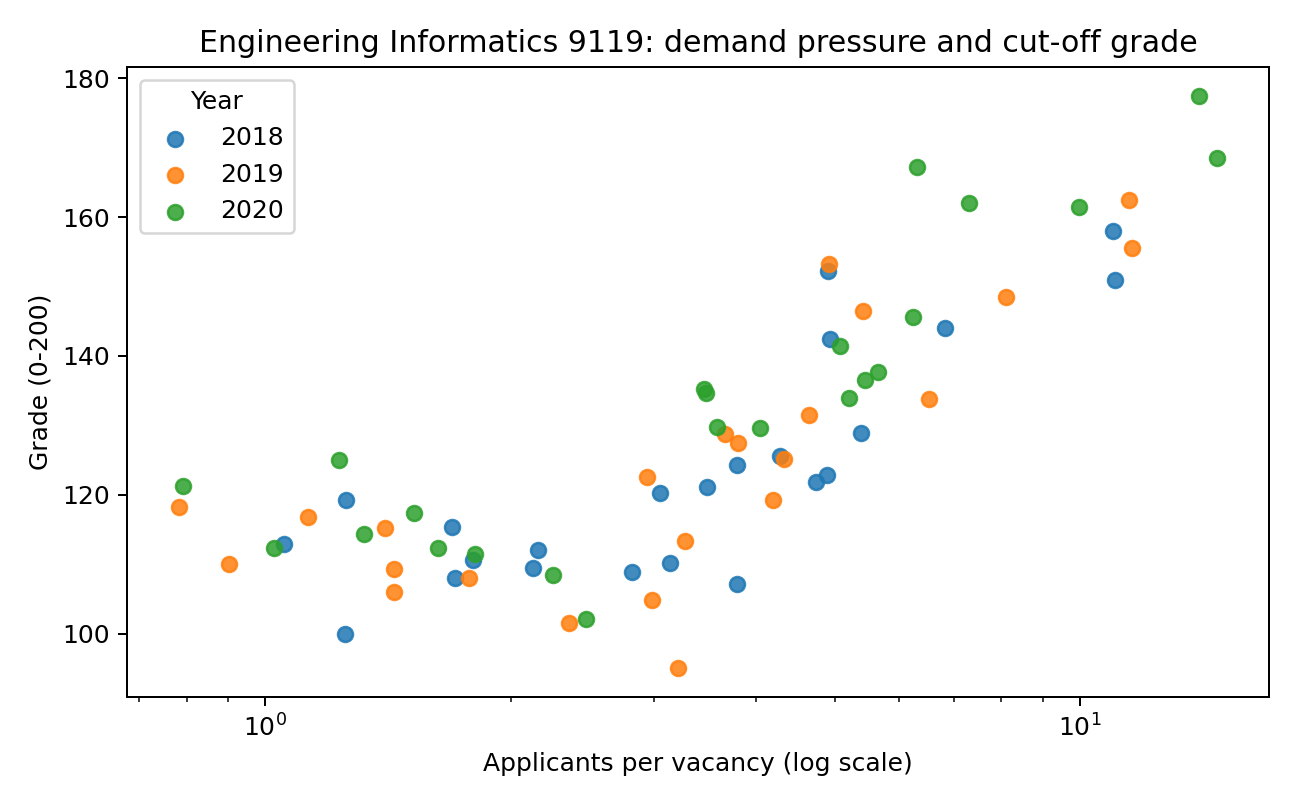
\includegraphics[width=0.82\textwidth]{../figures/study_b/course9119_demand_vs_cutoff.png}
\caption{Applicants per vacancy and general-contingent cut-off for the same course across 23 institutions. The horizontal axis is logarithmic.}
\end{figure}

\subsection{Institution structure and out-of-year prediction}
With only a linear year term, the pooled cut-off model has $R^2=0.058$; adding log
applicants per vacancy raises it to 0.674. For the mean placed grade, the corresponding
values are 0.105 and 0.679. Institution fixed effects alone with the year term raise
$R^2$ to 0.953 for the cut-off and 0.958 for the mean grade. Adding demand on top of
that structure raises these to 0.973 and 0.976, incremental gains of 0.020 and 0.018.

This decomposition shows that the strong cross-sectional relation coexists with
persistent institution differences. Demand and institution structure are not competing
explanations in a simple additive sense: institutions with persistently high demand
also tend to have persistently high entry grades.

The same pattern appears in leave-one-year-out prediction. For the institution-and-year specification, adding demand reduces mean held-out RMSE from 9.10 to 7.49 grade
points for the cut-off and from 6.51 to 5.13 for the mean placed grade. Demand therefore
contains information that is not exhausted by institution identity in this pilot.

The evidence is deliberately restricted to one exact course. It does not establish the
share of grade variation explained by demand across Portuguese higher education as a
whole, and it does not evaluate ranking information.

\section{Reliability conditions}
The empirical results are reported only after the following checks:
\begin{itemize}
\setlength{\itemsep}{0pt}
\setlength{\parskip}{0pt}
\item each observed year contains the same 23 source areas and reconciles exactly to
published national controls;
\item the missing 2019 field composition remains missing, and non-consecutive
observations are not labelled year-on-year changes;
\item the 2020--2021 exclusion sensitivity is evaluated separately;
\item the demographic series covers every required preceding population year and uses
one consistent INE/PORDATA source;
\item the cohort proxy is labelled distinctly from an exact age-18 denominator;
\item all 23 duplicated 2019 course-9119 observations agree across the two comparative
publications before canonicalisation;
\item the matched-course panel contains the same 23 institutions in all three years.
\end{itemize}
These checks constrain interpretation but do not create a causal design.

\section{Discussion}
The medium-run evidence does not support a simple statement that absolute first-phase
STEM placements have continuously declined since 2017. The 2026 all-STEM count is
higher than both the 2017 and 2023 counts, and the 2025 contraction is followed by a
large rebound. Yet that observation is only one margin. The all-STEM share of national
placements is slightly lower than in 2017, first-choice pressure has weakened, and the
broad-cohort-normalised aggregate is approximately flat between the endpoints.

The component results are more informative than the aggregate. Natural sciences,
mathematics and statistics are lower in both raw and normalised terms. ICT expands
strongly from its 2017 base. Engineering, manufacturing and construction rises in raw
counts but only modestly after demographic normalisation. Consequently, ``fewer
placements'', ``lower relative share'', ``weaker first-choice pressure'' and ``lower
placements relative to cohort scale'' are distinct empirical statements.

The matched-course results add a second distinction. Applicants per vacancy are strongly
associated with entry grades when the programme is held exactly fixed, but the amount
of cross-institution variation accounted for is neither constant nor complete. Much of
the persistent variation is also absorbed by institution effects, while demand still
improves held-out-year prediction. A broad claim about demand therefore requires both
matched-programme comparisons and replication across fields, rather than a single
pooled correlation.

The remaining limitations are substantive. The broad-area field composition is not
observed for 2019, the medium-run series begins only in 2017, and broad-area tables do
not contain total programme applications. The demographic denominator is a broad
cohort proxy rather than the preferred exact age-18 series. Degree reforms also make
longitudinal programme comparability a separate measurement problem. The next stage
therefore requires a historical programme-by-institution panel across many fields
before formal long-run diagnostics or a general Study B demand decomposition are warranted.

\section{Conclusion}
Between 2017 and 2026, raw registered STEM placements rise by 9.0\%, their share of
all first-phase placements falls by 0.64 percentage points, and the broad-cohort-
normalised endpoint rate rises by only 1.3\%. Component paths diverge substantially,
so the medium-run evidence cannot be represented by one claim of continuous aggregate
decline. In the separate matched-course analysis, applicants per vacancy explain a
large but variable share of cross-institution entry-grade differences and improve
out-of-year prediction even after institution effects. That pilot is not a general
Study B result. The 1997--2026 programme-level Study A test, regionality, rankings and
the R\&D pipeline remain unresolved empirical questions.

\end{document}
